In assembly, computation and readout of single atoms, laser cooling and trapping techniques play a central role. This chapter will give some background on how this technique works, and how we intend to apply it onto strontium (Sr).


\section{Magneto Optical Trap}

The workhorse for producing clouds of ultra-cold atom is the 3D magneto optical trap (MOT). In essence it, consists of three sets of counter-propagating beams as well as as magnetic field gradient, together providing a dampening as well as a confining force. 

\subsection{Doppler Cooling}

Consider an atom with ground state $\ket{g}$ and excited state $\ket{e}$ separated by an energy splitting $\hbar \omega_0$. We drive a laser with omega $\omega$ that is near resonant, but \emph{detuned} slighty from the transition by an amount $\delta$:

\begin{equation}\label{detuning}
	\delta = \omega - \omega_0
\end{equation}

It will turn out that the detuning is one of the most important parameters in laser cooling. Typically, $\delta <0$. Because of the doppler effect, the atom 'sees' a slightly different light frequency depending on its velocity $v$ according to $\delta'=\delta+kv$ and it is possible that the laser becomes resonant: $\delta' = \omega_0$, causing the atom to absorb a photon absorbing momentum $\hbar k$ and promoting an electron to the excited state. When spontaneous emission causes the atom to fall back in a time $\tau = 1/\gamma$ where $\gamma$ is the linewidth of the transition, the electron is decayed back to the ground state, but the emitted photon is emitted in a random direction. This can be repeated many times per second at a scattering rate $\Gamma_{sc}$ \cite{Metcalf1999}

\begin{equation}\label{eq:ScatteringFrequency}
	\Gamma_{sc} = \frac{ \gamma s_0 /2}{1+s_0+\left[2(\delta+ k v)/\gamma\right]^2},
\end{equation}

where $s_0 = I/I_{sat}$ is the saturation parameter as a function of the light intensity $I$ for saturation intensity $I_{sat} = \hbar c \gamma \pi/3\lambdaup^3$ for wavelength $\lambda$ and linewidth $\gamma$. Because the absorption occurs in a fixed direction and the emission is a random event, the atom will experience a net force scatering force $F = \hbar k \Gamma_{sc}$.

\subsection{Optical Molasses}

We can reflect the laser beam using a mirror, such that the force works in both directions of the coordinate which we call $z$. The total force from both contributions from \cref{eq:ScatteringFrequency} is \cite{Kowalski2010}

\begin{equation}\label{eq:OpticalMolasses}
	F = \frac{\hbar k \gamma s_0}{2}\left\{\
	\left[1 + s_0 + 4\frac{(\delta+kv)^2}{\gamma^2}\right]^{-1}+
	\left[1 + s_0 + 4\frac{(\delta-kv)^2}{\gamma^2}\right]^{-1}
	\right\}
\end{equation}

We have plotted the result of \cref{eq:OpticalMolasses} as a function of velocity in units of $\hbar / k$ to make it dimensionless. Contributions of both beams, as well as their total force are shown in units of $\hbar k \gamma$. Doing a series expansion to first order around $v = 0$. For $\delta<0$ we find we can linearize the force $F$ as 

\begin{figure}
\centering
	\begin{minipage}{.49\textwidth}
		\centering
		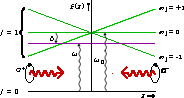
\includegraphics[width=\linewidth]{figures/OpticalMolasses.pdf}
	\end{minipage}
	\begin{minipage}{.48\textwidth}
		\centering
		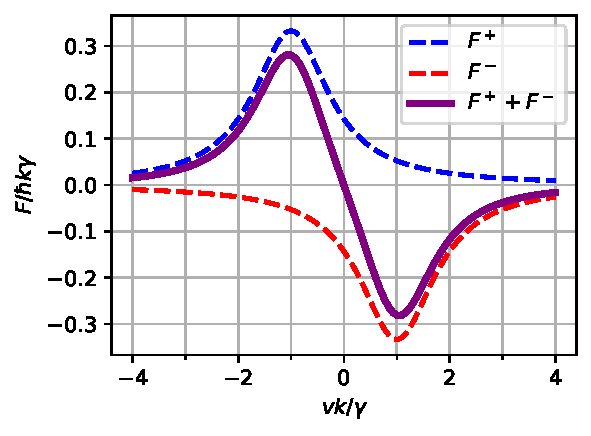
\includegraphics[width=\linewidth]{figures/MOTplot.pdf}
	\end{minipage}
	\caption{a) Concept of optocal molasses in 1D. Atomic frequency is detuned from the atomic transition by $\delta<0$. Because of the linear magnetic field, at some displacement the $m_j=-1$ atoms become resonant with only $\sigma^+$ light because of selection rules, and vice versa. b) Cooling force from a magneto-optical trap. Contributions from the $F^+$, $F^-$ and the total force are shown for $\delta = -\gamma$ and $I/I_0 = 2.$}
		\label{fig:MOTdamping}
\end{figure}

\begin{equation}\label{eq:linearize}
	F \approx - \hbar k^2 s_0 \frac{-2\delta/\gamma}{\left[1+s_0+(2\delta/\gamma)^2\right]^2} \equiv -\beta v
\end{equation}

Where $\beta$ is the slope of the scattering force around $v=0$. Apparently, the resulting force has a dampening character on the velocity, which if applied in all 3 dimensions can effectively cool atoms. 

The treatment so far would suggest that this can be used to cool atoms to temperatures of absolute zero. This is not the case, as the random character of the scattering force means the atom fluctuate around the equilibrium velocity according to a Brownina motion. For $\delta=-\gamma/2$, $\beta$ is at a maximum, yielding the lowest possible temperature achievable using Doppler cooling called the Doppler temperature $T_D$

\begin{equation}\label{eq:DopplerTemperature}
	T_D = \frac{\hbar}{2k_b} \gamma.
\end{equation}

where $k_b$ is Boltzmann's constant. Apparantly, this cooling limit is only dependent on the linewidth of the transition $\gamma$, apart from physical constants. This result will be used later in \cref{sec:Sr}.

\subsection{Magnetic Trapping}

Apart from cooling the atoms, we want to trap them at a specific location to increase the density of atoms. We can use the Zeeman effect for this, which tells us the atomic energy levels will be split an amount $\Delta E$ according to \cite{Griffiths2004}

\begin{equation}\label{eq:Zeeman}
	\Delta E = \mu_{\emph{B}} g_J m_j B,
\end{equation}

where $B$ is the Bohr magneton, $g_J$ the Landé g-factor, $m_j$ is the magnetic quantum number and $B_{\text{ext}}$ the applied magnetic field. The magnetic field is tuned in such a way that is is linear in all 3 dimensions and zero at the center of the MOT by using a set of magnetic field coils in anti-Helmholtz configuration. Because of the Zeeman splitting, the chance of the atoms coming in resonance with the laser vary with the position from the origin acoording to 

\begin{equation}\label{eq:DetuningFull}
	\delta' = \delta + k v - \frac{\mu'B}{\hbar}
\end{equation}

To ensure that atoms only absorb momentum kicks in the right direction, the laser beams are circularly polarized: $\sigma^+$ from the left and $\sigma^-$ from the right. Because the sign of the Zeeman shift is dependent on the magnetic quantum number $m_j$, selection rules prescribe. For 3 dimensions the force becomes

\begin{equation}\label{eq:MOTfull}
	\frac{F}{\hbar k \gamma s_0} = \frac{1}{2}\left\{\
	\left[1 + s_0 + 4\frac{(\delta+kv+\mu'B/\hbar)^2}{\gamma^2}\right]^{-1}+
	\left[1 + s_0 + 4\frac{(\delta-kv-\mu'B/\hbar)^2}{\gamma^2}\right]^{-1}
	\right\}
\end{equation}

Where $\mu' = (g_e m_e-g_g m_g)\mu_B$ is the effective magnetic moment for the transition \cite{Kowalski2010}. Expanding \cref{eq:MOTfull} around $(v,z) = (0,0)$, keeping only first order terms, extending the same concept to the other two dimenions yields finally

\begin{equation}\label{eq:ForceMOT}
	F_{\text{MOT}}(z,v) \approx -\beta v - \kappa z.
\end{equation}

Where $\beta$ is the same we found in \cref{eq:linearize} and $\kappa \equiv \mu' \beta /\hbar k \cdot \partial B/\partial z$. Apart from the dampening force, a force with Hookian charcter arises for linear magnetic field gradient as well. These are the two ingredients for producing high density cold atom clouds. 



\section{Stontium}\label{sec:Sr}

Historically, people started laser cooling experimentation on group 1 or alkali atoms (Na, Rb, Cs). Because they only have one valence electron, the level structure is relatively straightforward. Also, diode lasers are available for their transition frequencies. This work contains trapping of alkali earth atoms explained in \cref{ch:implementation}.

However, also group 2 atoms, also called alkali-earth (and similar atoms like Yb) are a possible candidate. Because of their two valence electrons, the level structure is much more complicated, making laser cooling harder, but possibly also opening up new possiblities. The element we wish to use for our new machine in Eindhoven is Sr. For a more extensive coverage of Sr, the reader is refered to \cite{Stellmer2013}. Three of them are bosonic, with ${}^{88}$Sr being the most abundant at $\sim82.6\%$. There is one stable fermionic isotype: ${}^{87}$Sr has a nuclear spin of $I=9/2$ and an abundance of $\sim7.0\%$ \cite{Coursey1999}. This work is on \textsuperscript{88}Sr. Because of the lack of hyperfine structure it simplifies a whole lot of things, but in principle one can work on all isotopes in the same machine as the energy splitting between the isotopes is in the MHz regime. 

Strontium is also used in the best atomic clocks in the world \cite{Bloom2014}, some for of the same reasons that it is a good candidate candidate for quantum computing, which we will discuss here. 

\subsection{Relevant Transitions}

A simplified version of the level diagram of \textsuperscript{88}Sr is shown in \cref{fig:SrLevel}. The notation is $(n_1l_1 n_2l_2)^{2S+1}L_J$ where $n_{1,2}$ is the principal and $l_{1,2} = s, p, d, \ldots$ the azimuthal quantum number. Furthermore $S$, $L$ and $J$ are the total spin, orbital angular momentum and total angular momentum respectively \cite{Cowan1981}.  This level scheme shows 6 out of 7 lasers to be used in this experiment. 

\begin{itemize}
	\item 461 nm. Broad transition, meaning a strong scattering force (\cref{eq:ScatteringFrequency} and short lifetime and quick cycling frequency. This is useful to slow down the hot atomic beam coming from the oven, as well as catching the atoms in a so called blue MOT with 'hot' temperatures of $\sim$ 1 mK.)
	
	\item 689 nm. Being much narrower than the blue transition, its Doppler temperature \cref{eq:DopplerTemperature} is much lower at $179$ nK, although in practice cooling is limited by the recoil limit to some $\sim 1$ $\mu$K \cite{Boyd2007,Stellmer2013}.
	
	\item 698 nm. The ultra-narrow clock transition ($\gamma = 1$ mK). Used in atomic clocks because of its spectroscopic accuracy \cite{Bloom2014}. It will turn out that this feature can be put to good use in quantum computers as well, and we will use it do coherently 'drive' the qubits between the qubit basis states. More about this in \cref{sec:QubitScheme}
	
	\item 679, 688 and 707 nm. All repump lasers. 707 and 688 are used to cycle back atoms from ending up in ${}^3P_2$ from the decay channel showed by the grey dotted line in \cref{fig:SrLevel}. 679 is used to prevent repump leaks to ${}^3P_0$ \cite{Stellmer2013,Xu2003}.
\end{itemize}

One wavelength is not shown, which is in fact the laser that will supply the most amount of power. This is the trapping laser, which determines the amount of single atoms and therefore qubits the machine can house. Using 813 nm, it is detuned so far from resonance that is not shown in \cref{fig:SrLevel} This wavelength gives the same light shift for ${}^1S_0$ and ${}^3 P_0$. This will be explained more thoroughly in \cref{sec:OpticalDipoleTrap}. 

\begin{figure}
	\centering
	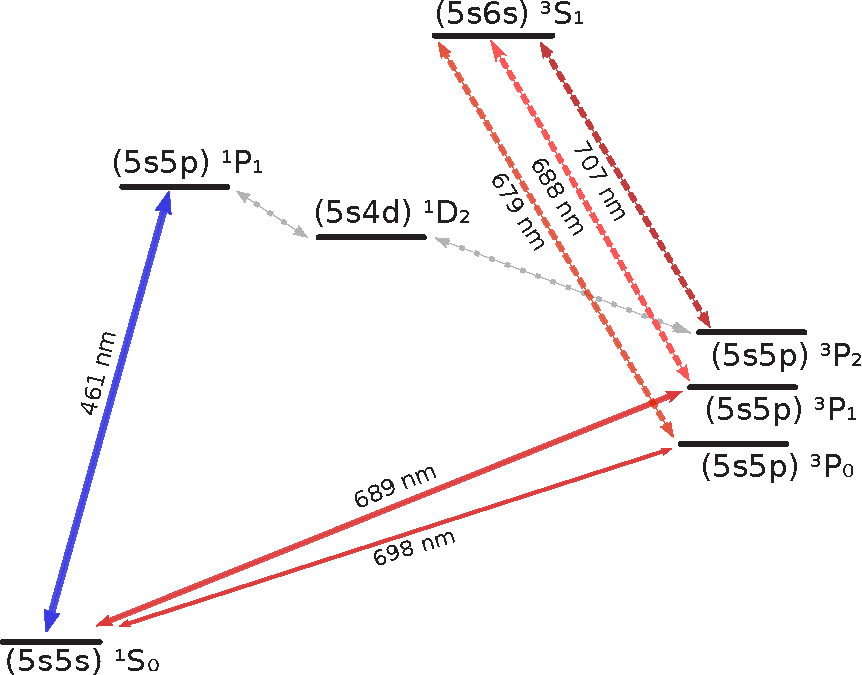
\includegraphics[width=0.55\linewidth]{figures/SrLevel.pdf}
	\caption{Simplified level scheme for \textsuperscript{88}Sr. Shown: blue transition for initial slowing and cooling. Narrower 689 nm transition of the red MOT, and the \textsuperscript{1}S\textsubscript{0} - \textsuperscript{3}P\textsubscript{0} clock transition, which we will be used to drive the qubits. To increase density and trap lifetime 3 repump lasers are used. Not shown: 813 nm dipole trapping laser because it is driven far off-resonant. Energies not to scale. Figure made by Ivo Knottnerus.}
	\label{fig:SrLevel}
\end{figure}

\subsection{Laser Cooling and Trapping of Sr}

Because of the melting temperature of Sr is $777$ ${}^{\circ}$C, to get any relevant vapor pressure, the Sr is heated in an oven after which it sublimates. To obtain a small atomic beam divergence, the atoms are directed along abundle of capillary tubes with high aspect ratio \cite{Stellmer2013}. 

Because of the oven, the atoms are moving way too fast to be efficiently captured by the MOT. Therefore, they are slowed by a Zeeman slower. This is a device similar to a MOT, but designed to cool only in one direction. A red-detuned laser is propagating in opposite direction of the atomic beam. A spatially varying magnetic field ensures a wide range of velocities is at some point resonant with the laser according to \cref{eq:DetuningFull}. 

Depending on the length of the Zeeman slower, only a fraction of the atoms will be slowed. To seperate the hot from the cool atoms (the former are unwanted in a vacuum chamber) a deflection stage is used. The blue transition of Sr is used for this stage because of the strong scattering force. The Zeeman slowing and deflection stage is explained more elaborately in the thesis of Rik van Herk \cite{Herk2022}.

After the deflection stage, the atomic beam enters a glass cell. The advantage of using a glass cell is that is allows for the maximum amount of optical axis. To allow for longer trap survival times, the glass cell has ultra-high vacuum (UHV) which is separated from the stages preceding it by a differential pumping stage. 

\begin{figure}
	\centering
	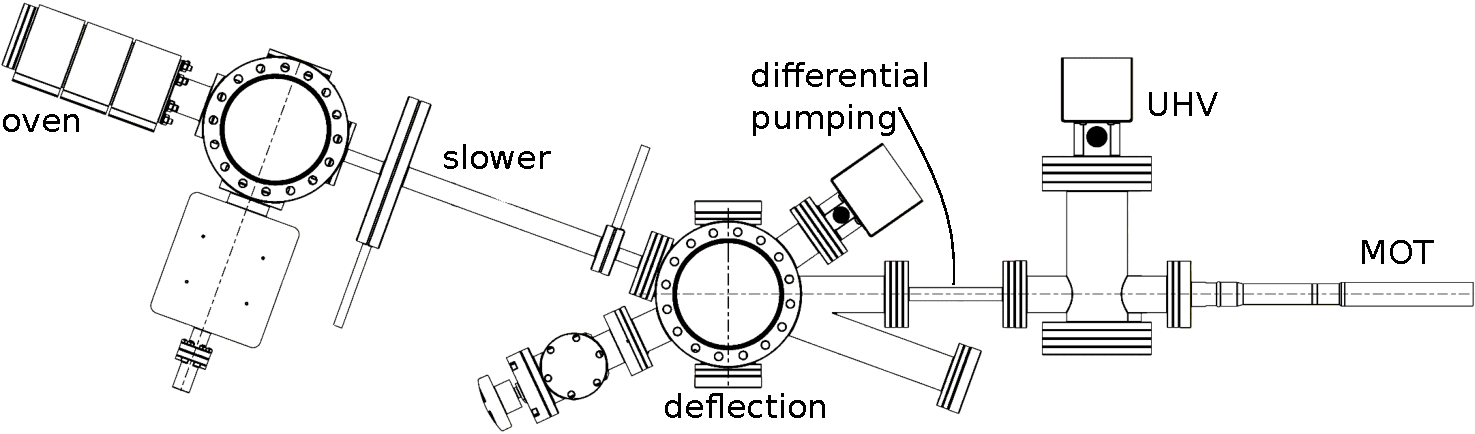
\includegraphics[width=0.9\linewidth]{figures/SrLoading.pdf}
	\caption{Sketch of the vacuum atom source design and vacuum chambers. Starting from the oven, the atomic beam traverses a Zeeman slower, deflection stage and differential pumping stage before ending in the glass cell (MOT, right). Figure by Patrick de Laat.}
	\label{fig:SrLoading}
\end{figure}

\subsection{Stontium as a Qubit}\label{sec:QubitScheme}

The main reason we want to use strontium atoms for the quantum processing unit is the ${}^3P_0$ state and its very long life time. The clock transition is forbidden according to selection rules, and only opens up after applying a magnetic field for the \textsuperscript{88}Sr isotope, after which the lifetime is in the order of $\sim 100$ s. On the timescales of the operation of a quantum computer, we can therefore consider ${}^3P_0$ a 'second ground state'. 

We aim to define the two clock states as our qubit manifold, such that we have:

\begin{equation}\label{eq:QubitManifold}
	\big\{\ket{0},\ket{1}\big\} = 
	\left\{
		\ket{{}^1S_0}, \ket{{}^3P_0} 
	\right\}
\end{equation}

Such that we have two long-lifetime states with a extremely narrow transition between them such that we can coherently drive between the qubit states. Because both states are 'ground' states, this type of scheme is called $\ket{gg}$ \cite{Wu2021}. To entangle the qubits, Rydberg dressing can be used \cite{Wu2021} where a small part of a Rydberg state $\ket{r}$ is admixed in one of the ground states. 

\begin{equation}\label{eq:RydbergDressing}
	\ket{\psi} \sim \ket{g} + \epsilon \ket{r}
\end{equation}

The degree dresing is tuned by the (small) dressing parameter $\epsilon \propto \Omega / 2\delta$ where $\Omega$ is the Rabi frequency of the laser and $\delta$ the usual detuning. A Rydberg state is an electronic state with very high principal quantum number $n$. Rydberg atoms are physically larger, as the electron orbit scales $\propto n^2$ \cite{Gallagher1994}. As a result of these exagerrated electron orbit sizes, neighboring atoms can 'feel' each other. For example, the van der Waals interaction coefficient scales as $\propto n^{11}$ \cite{Gallagher1994}. 

Other qubit implementations than the one above are possible as well. For example, \cite{Barnes2021} uses the fermionic ${}^{87}$Sr and maps the qubit states onto the nuclear spin states $\ket{{}^1S_0, F=9/2, m_F = -9/2}$ and $\ket{{}^1S_0, F=9/2, m_F = -7/2}$ nuclear magnetic spin states. 


\section{Optical Dipole Traps}\label{sec:OpticalDipoleTrap}

Now that the qubit manifold is known, we will talk about how to experimentally trap these qubits. While magneto optical traps are excellent for producing cloulds of ultracold atoms, the constant photon scattering is unwanted during qubit operation. Therefore, after the atom cloud is cooled in the MOT, the MOT is typically overlapped with another type of trap: the optical dipole trap (ODT). An ODT uses far off-resonant light and is therefore much weaker. However, because the light is off-resonant, such that scattering events are kept to a minimum and is thus non-destructive for coherence. 

\subsection{Dipole Force}\label{sec:DipoleForce}

The light field $\mathbf{E}$ will induce a dipole moment $\mathbf{p}$ in the atom according to 
	
\begin{equation}\label{eq:DipoleMoment}
	\mathbf{p} = \alpha \mathbf{E}
\end{equation}

in turn, the dipole potential will interact with the electric field leading to and an interaction dipole potential $U_{dip}$

\begin{equation}\label{eq:DipolePotential}
	U_{\text{dip}}(\mathbf{r}) = -\mathbf{p}\mathbf{E} = 
	-\frac{1}{2} \left\langle \mathbf{p}\mathbf{E} \right\rangle = \frac{\operatorname{Re}(\alpha)}{2\epsilon_0 c} I(\mathbf{r})
\end{equation}

where we have averaged the rapidly oscillating phase terms of the light, giving the factor $1/2$ and furthermore $I(\mathbf{r}) = |\mathbf{E}(\mathbf{r})|^2/(2\epsilon_0 c)$. An additional factor $1/2$ comes in because the dipole moment is induced and not permanent. The gradient of \cref{eq:DipolePotential} gives rise to the dipole force:

\begin{equation}\label{eq:DipoleForce}
	\mathbf{F}_{\text{dip}}(\mathbf{r}) = - \frac{\operatorname{Re}(\alpha)}{2\epsilon_0c}\nabla I(\mathbf{r})
\end{equation}

\cref{eq:DipoleForce} tells us that in order to maximize the dipole force, one has to maximize the gradient of the light intensity profile. This can be done by focussing the laser to the smallest possible spot, in order to achieve the highest possible dipole force. The scattering rate from the ODT can be found by averaging over the derivative of the dipole moment with the electric field 

\begin{equation}
	\Gamma_{sc}(\mathbf{r}) = \frac{\left\langle \mathbf{p} \mathbf{E} \right\rangle}{\hbar \omega}
	 = \frac{\operatorname{Im}(\alpha)}{\hbar \epsilon_0 c} I(\mathbf{r}) 
\end{equation}

These expressions are true for any atom in a potential. The task that remains is finding the polarizability $\alpha$. As a staring point, we will consider the electron as a harmonic oscillator with a damping coefficient. The dampening yields the polarizability, which for alkali atoms like Rb is accurate to within a few percent: 

\subsection{Classical}

In the classical picture, we assume a classical light field $\mathbf{E}(z,t) =\epsilon_0 E_0 / 2 \left(	
	\exp{(i \omega t)}+\exp{(-i \omega t)}
	\right)\hat{\mathbf{z}}$, and a quantized atom potential. 

\begin{equation}
	\alpha = 
\end{equation}


\begin{figure}
	\centering
	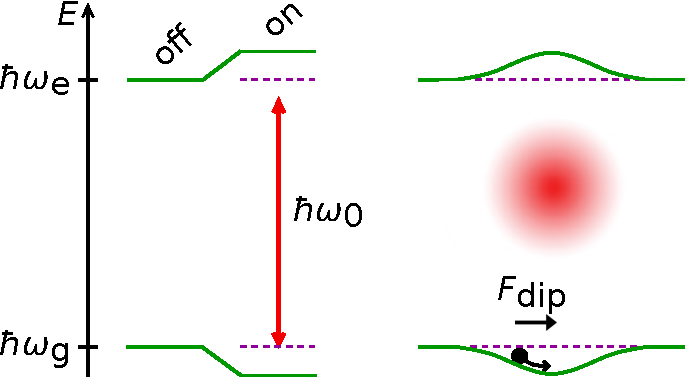
\includegraphics[width=.45\linewidth]{figures/LightShift.pdf}
	\caption{Light shift when the off-resonant laser is turned on, as well as the spatially varying light shift for a Gaussian beam. Figure adapted from \cite{Grimm2000}}
	\label{fig:DipoleForce}
\end{figure}




\section{Gaussian Beams}\label{sec:GaussianBeams}

Optical tweezer are in essence tightly focussed laser beams. We will briefly revisit the description of the commonly used laser beam because it is used throughout this work. Starting from Maxwell equations, one can derive under paraxial approximation a description of the transverse electromagnetic mode (TEM\textsubscript{00}) \cite{Leeuwen2017} for the electric field $E$. This Gaussian beam is most conveniently written down in cilindrical coordinates $\{r,z\}$:

\begin{equation}\label{GaussianBeam}
	E(r,z) = \frac{w_0}{w(z)} \exp{\left(\frac{-r^2}{w^2(z)}\right)} \exp{\left[-ikz-i\frac{kr^2}{2R(z)} - i\psi(z)\right]},
\end{equation}

with parameters

\begin{equation}
	k = \frac{2\pi}{\lambdaup}, \quad 
	w(z) = \sqrt{w_0 + \frac{z^2}{z_R^2}}, \quad \text{and} \quad
	R(z) = z \left(1 + \frac{z^2}{z_R^2}\right).
\end{equation}

Respectively, the wave number in terms of the wavelength $\lambdaup$, the beam waist, the radius where the field drops $1/e$ in terms of $w(z)\equiv w_0$ and $R(z)$ is the wavefront curvature. Finally $\psi(z)$ is an extra phase term originating from the curvature of the wavefront known as the Gouy phase. We find the intensity of the Gaussian beam by taking the absolute value squared:

\begin{equation}\label{GaussianBeamIntensity}
	I(r,z) = I_0 \frac{w_0^2}{w^2(z)} \exp{\left(\frac{-2r^2}{w^2(z)}\right)}
\end{equation}

A sketch of a Gaussian beam profile is given in \cref{fig:GaussianBeam}, showing the $1/e$ field radius, or $1/e^2$ intensity radius $w_0$ and the Rayleigh range or depth of focus $z_R$. 

\begin{figure}
	\centering
	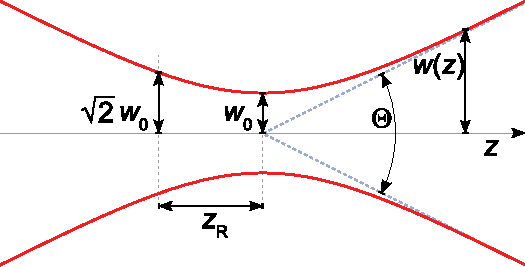
\includegraphics[width=0.4\linewidth]{figures/GaussianBeam.pdf}
	\caption{Gaussian beam profile and some key parameters used in this work, the beam waist $w_0$ and Rayleigh range $z_R$. Figure adapted from \cite{Hermans2009}.}
	\label{fig:GaussianBeam}
\end{figure}


\section{Loading Single Atoms}\label{sec:LoadingAtoms}

For the quantum register, an array of single atoms is needed. In order to do this, individual atoms from the cold atom cloud are loaded in optical tweezers, or tightly focused laser beams. We can write the dynamics of the number of atoms $N$ in the tweezer as \cite{Schlosser2002}

\begin{equation}\label{LoadingTweezer}
	\frac{\text{d}N}{\text{d}t} = \alpha - \gamma N - \beta N(N-1)
\end{equation}

where the first term $\alpha$ is the loading rate or the amount of Rb atoms entering the tweezer per second. Next, $\gamma$ is the atom loss as a result of collisions with the background gas. Lastly, $\gamma$ is a measure for the mainly 2 body loss as a result of light-assisted collisions. No additional laser is required for this, the MOT beams can be used for this purpose.  

We are interested in the case $\beta \gg \gamma$: the two-body collisions are dominant. We can now look at two distinct scenarios:

\begin{itemize}
	\item Starting from 0 atoms in the tweezer: an additional atom entering will now load the tweezer to $N=1$. 
	
	\item Starting from $N=1$: when an additional atom is loaded, the atoms will immediately kick out each other because of the tiny tweezer volume and strong light intensity from the MOT beams. 
\end{itemize}

Apparently, a loading event can lead to either 0 or 1 atom in the tweezer, both with $50\%$ probability. This is known as the collisional blockade effect. Experimentally demonstrated by \cite{Schlosser2001} and \cite{Schlosser2002} showed this effect to exits for 3 orders of magnitude in the loading rate $\alpha$.

Experimentally, $\beta \gg \gamma$ can be keeping $\gamma$ to a minimum by going to the ultra high vacuum regime. We intent to go to a pressure of the order of $10^{-10}$ mbar. In addition $\beta$ is maximized by going to high light-intensities and small trapping volumes. 